\documentclass[11pt,a4paper]{article}
\usepackage[T1]{fontenc}
\usepackage[utf8]{inputenc}
\usepackage[french]{babel}
\usepackage{lmodern}
\usepackage{microtype}
\usepackage[margin=2.2cm]{geometry}
\usepackage{amsmath,amssymb,amsthm,mathtools}
\usepackage{icomma}
\usepackage{booktabs,tabularx,array}
\usepackage{xcolor}
\usepackage{tikz}
\usetikzlibrary{patterns,positioning,arrows.meta,decorations.pathreplacing,shapes.geometric}
\usepackage{pgfplots}
\pgfplotsset{compat=1.18}
\usepackage[most]{tcolorbox}
\usepackage{enumitem}
\usepackage[hidelinks]{hyperref}
\usepackage{caption}
\usepackage{float}
\usepackage{pdflscape}
\usepackage{pifont}

\definecolor{nyt}{HTML}{1F3B63}
\definecolor{wp}{HTML}{17695B}
\definecolor{gov}{HTML}{B42318}
\definecolor{nat}{HTML}{9A6212}
\definecolor{regnone}{HTML}{C6C2B8}
\definecolor{regnosuit}{HTML}{CBE2C3}
\definecolor{regnyt}{HTML}{F0C5BD}
\definecolor{regboth}{HTML}{F1D69B}

\newtcolorbox{cours}{colback=nat!6,colframe=nat!70,boxrule=0.5pt,arc=2pt,left=6pt,right=6pt,top=4pt,bottom=4pt,fonttitle=\bfseries\small,title=Lien avec le cours}
\newtcolorbox{resultat}{colback=wp!6,colframe=wp!70,boxrule=0.5pt,arc=2pt,left=6pt,right=6pt,top=4pt,bottom=4pt}
\newtcolorbox{intuition}{colback=nyt!4,colframe=nyt!50,boxrule=0.4pt,arc=2pt,left=6pt,right=6pt,top=3pt,bottom=3pt,fonttitle=\bfseries\small,title=Intuition}

\theoremstyle{definition}
\newtheorem{lemme}{Lemme}
\newtheorem{proposition}{Proposition}
\newcommand{\ind}[1]{\mathbf{1}_{\{\text{#1}\}}}
\newcommand{\E}{\mathbb{E}}
\setlength{\parindent}{0pt}
\setlength{\parskip}{5pt}
\captionsetup{font=small,labelfont=bf}

\newtcolorbox{erreur}{colback=gov!5,colframe=gov!70,boxrule=0.5pt,arc=2pt,left=6pt,right=6pt,top=4pt,bottom=4pt,fonttitle=\bfseries\small,title=Erreur}
\newtcolorbox{discuter}{colback=nat!6,colframe=nat!70,boxrule=0.5pt,arc=2pt,left=6pt,right=6pt,top=4pt,bottom=4pt,fonttitle=\bfseries\small,title=À discuter}
\newtcolorbox{simple}{colback=nyt!4,colframe=nyt!50,boxrule=0.4pt,arc=2pt,left=6pt,right=6pt,top=3pt,bottom=3pt,fonttitle=\bfseries\small,title=En mots}
\newcommand{\T}[1]{\textcolor{nyt}{#1}}
\newcommand{\W}[1]{\textcolor{wp}{#1}}
\newcommand{\N}[1]{\textcolor{gov}{#1}}


\newtcolorbox{reponse}{colback=wp!6,colframe=wp!70,boxrule=0.6pt,arc=2pt,left=7pt,right=7pt,top=5pt,bottom=5pt,fonttitle=\bfseries,title=Réponse à la consigne}
\newcommand{\strip}[4]{% label, max, segments {start/end/color/text}, current
\begin{tikzpicture}[x=11cm/#2,y=1cm]
\node[anchor=west,font=\small] at (0,0.62) {#1};
\foreach \a/\b/\c/\t in {#3}{\fill[\c] (\a,0) rectangle (\b,0.42); \node[font=\scriptsize] at ({(\a+\b)/2},0.21) {\t};}
\draw[black!60] (0,0) rectangle (#2,0.42);
\draw[gov,line width=1.6pt] (#4,-0.1)--(#4,0.52); \node[font=\scriptsize,text=gov,below] at (#4,-0.08) {valeur : #4};
\node[font=\scriptsize,below] at (0,-0.05) {0}; \node[font=\scriptsize,below] at (#2,-0.05) {#2};
\end{tikzpicture}}
\colorlet{cboth}{nat!45}\colorlet{cnyt}{gov!30}\colorlet{cnosuit}{wp!30}\colorlet{cnone}{black!18}\colorlet{cnc}{wp!55}

\title{\textbf{Pentagon Papers}\\[3pt]\large Réponses aux cinq consignes : joueurs, issues, seuils, secret et équilibre}
\author{Travail de théorie des jeux, groupe 5--6 · ECGEB366 « Stratégies économiques »}
\date{}

\begin{document}
\maketitle
\vspace{-1.1cm}

\begin{resultat}
\textbf{Ce document} répond aux cinq consignes de l'énoncé avec le modèle du groupe : le calcul des gains de l'arbre (document « Le jeu des Pentagon Papers : les gains des 7 issues »), la fiche des formules des seuils et intervalles, et le simulateur \texttt{sequential-game-sim.vercel.app}. Tous les chiffres ci-dessous ont été recalculés avec ce modèle.

\textbf{En une phrase.} Avec les valeurs du groupe, l'équilibre parfait en sous-jeux reproduit 1971 : le Times publie, Nixon le poursuit, le Post publie à son tour, Nixon le poursuit aussi ($O_1$, gains espérés $(6\ ;\ 0{,}5\ ;\ -3{,}5)$). Ce scénario se réalise tant que $53{,}3\,\%\le p<80\,\%$ (avec $q=50\,\%$).
\end{resultat}

\subsection*{Les valeurs du groupe}
\begin{center}
\small
\begin{tabular}{@{}llr@{\qquad}llr@{}}
\toprule
\multicolumn{3}{@{}l}{\T{\textbf{New York Times}}} & \multicolumn{3}{l@{}}{\N{\textbf{Administration Nixon}}} \\
$B_T$ & bénéfice s'il publie tout & 10 & $D$ & dommage si tout sort & 5 \\
$c_T$ & coût de son procès & 1 & $k_T$ & coût d'un procès contre le Times & 1 \\
$S_T$ & sanction s'il perd & 5 & $k_W$ & coût d'un procès contre le Post & 1 \\
\multicolumn{3}{@{}l}{\W{\textbf{Washington Post}}} & $R$ & bonus si le secret est gardé & 10 \\
$B_W$ & bénéfice s'il publie tout & 10 & \multicolumn{3}{l@{}}{\textcolor{nat}{\textbf{Juges (pas des joueurs)}}} \\
$c_W$ & coût de son procès & 3 & $q$ & le juge local refuse la censure & 50\,\% \\
$S_W$ & sanction s'il perd & 5 & $p$ & la Cour suprême donne raison aux journaux & 60\,\% \\
 & & & $\theta$ & part publiée avant une censure & 0 \\
\bottomrule
\end{tabular}
\end{center}

% =====================================================================
\section{Consigne 1 : les joueurs et l'ordre dans lequel ils interviennent}

\subsection{Trois joueurs, et des juges qui n'en sont pas}
Un \emph{joueur} choisit une action pour servir son intérêt et reçoit un gain. Trois acteurs remplissent ces deux conditions.

\begin{figure}[H]
\centering
\begin{tikzpicture}[card/.style={draw=#1,line width=1pt,fill=#1!6,rounded corners=4pt,text width=4.3cm,align=left,font=\small,inner sep=6pt,minimum height=2.5cm}]
\node[card=nyt] (T) at (0,0) {\textbf{\T{New York Times}}\\ Choisit : publier ou non.\\ Veut : le scoop, sans procès ni sanction.};
\node[card=wp] (W) at (5,0) {\textbf{\W{Washington Post}}\\ Choisit : publier ou non (en relais ou seul).\\ Veut : publier lui aussi, mais risque gros.};
\node[card=gov] (N) at (10,0) {\textbf{\N{Administration Nixon}}\\ Choisit : poursuivre en justice ou laisser faire.\\ Veut : garder le secret à moindre coût.};
\node[draw=nat,dashed,line width=0.9pt,fill=nat!6,rounded corners=4pt,text width=13.6cm,align=center,font=\small,inner sep=6pt] at (5,-2.4) {\textbf{\textcolor{nat}{Les juges : pas des joueurs}} (ni gain, ni stratégie). Leurs verdicts sont des \textbf{probabilités} qui modifient les gains des trois joueurs :\\ juge local : refuse la censure avec $q$ \quad·\quad Cour suprême (saisie seulement si les \emph{deux} journaux sont poursuivis) : donne raison aux journaux avec $p$.};
\end{tikzpicture}
\caption{Les trois joueurs et le rôle des juges. Ellsberg n'est pas un joueur non plus : il a déjà remis les documents quand le jeu commence.}
\end{figure}

\subsection{L'ordre des décisions}
\begin{figure}[H]
\centering
\begin{tikzpicture}[x=2.7cm,
  st/.style={draw=#1,fill=#1!10,line width=1pt,rounded corners=3pt,font=\small,align=center,inner sep=5pt,text width=2.2cm,minimum height=1.25cm},
  ar/.style={-{Stealth[length=3mm]},line width=1pt}]
\node[st=nyt] (a) at (0,0) {\textbf{1. Times}\\publie ?};
\node[st=gov] (b) at (1,0) {\textbf{2. Nixon}\\poursuit le Times ?};
\node[st=wp]  (c) at (2,0) {\textbf{3. Post}\\publie à son tour ?};
\node[st=gov] (d) at (3,0) {\textbf{4. Nixon}\\poursuit le Post ?};
\node[st=nat] (e) at (4,0) {\textbf{5. Juges}\\verdicts ($q$, $p$)};
\draw[ar] (a)--(b); \draw[ar] (b)--(c); \draw[ar] (c)--(d); \draw[ar,dashed] (d)--(e);
\node[st=wp] (f) at (1,-1.9) {\textbf{3'. Post}\\publie seul ?};
\node[st=gov] (g) at (2,-1.9) {\textbf{4'. Nixon}\\poursuit le Post ?};
\draw[ar] (a.south) |- (f.west); \node[font=\scriptsize,left] at (0,-1.4) {si le Times se tait}; \draw[ar] (f)--(g);
\end{tikzpicture}
\caption{L'ordre du jeu. Chaque joueur voit tout ce qui a été fait avant lui : le jeu est séquentiel, à information complète et parfaite.}
\end{figure}

\begin{reponse}
\textbf{Joueurs} : le New York Times (T), le Washington Post (W) et l'administration Nixon (N). Les juges ne sont pas des joueurs : leurs verdicts sont deux probabilités, $q$ (juge local) et $p$ (Cour suprême), intégrées aux gains sous forme de gains espérés.

\textbf{Ordre} : Times $\to$ Nixon $\to$ Post $\to$ Nixon (puis les juges tranchent). Si le Times ne publie pas : Post $\to$ Nixon.

\textbf{Stratégies} : le Times décide à 1 nœud (2 stratégies), le Post à 2 nœuds (4), Nixon à 3 nœuds (8) : $2\times4\times8=64$ profils de stratégies.
\end{reponse}

% =====================================================================
\section{Consigne 2 : les résultats potentiels}

En suivant toutes les combinaisons de choix, on obtient \textbf{sept issues}, $O_1$ à $O_7$, classées ci-dessous selon les catégories de l'énoncé.

\begin{landscape}
\begin{center}{\large\bfseries Les sept issues et leur catégorie}\\[2pt]{\small Chaque feuille est une fin possible de l'histoire. Couleur du cadre : catégorie de l'énoncé.}\end{center}\vspace{-4pt}
\noindent\resizebox{\linewidth}{!}{\begin{tikzpicture}[x=1cm,y=1cm,lab/.style={font=\scriptsize,fill=white,inner sep=1pt,sloped},eq/.style={line width=1.8pt,draw=gov},br/.style={line width=0.6pt,draw=black!55}]
\draw[br] (0.4,-7.928125)--(2.6,-4.56875) node[lab,midway,above]{Publier};
\draw[br] (0.4,-7.928125)--(5.0,-11.2875) node[lab,midway,below]{Ne pas publier};
\draw[br] (2.6,-4.56875)--(5.0,-2.6875) node[lab,midway,above]{Poursuivre};
\draw[br] (2.6,-4.56875)--(9.6,-6.449999999999999) node[lab,midway,below]{Laisser faire};
\draw[br] (5.0,-2.6875)--(7.4,-1.075) node[lab,midway,above]{Publier};
\draw[br] (5.0,-2.6875)--(9.6,-4.3) node[lab,midway,below]{Ne pas publier};
\draw[br] (7.4,-1.075)--(9.6,0.0) node[lab,midway,above]{Poursuivre};
\draw[br] (7.4,-1.075)--(9.6,-2.15) node[lab,midway,below]{Laisser faire};
\draw[br] (5.0,-11.2875)--(7.4,-9.675) node[lab,midway,above]{Publier};
\draw[br] (5.0,-11.2875)--(9.6,-12.899999999999999) node[lab,midway,below]{Ne pas publier};
\draw[br] (7.4,-9.675)--(9.6,-8.6) node[lab,midway,above]{Poursuivre};
\draw[br] (7.4,-9.675)--(9.6,-10.75) node[lab,midway,below]{Laisser faire};
\fill[nyt] (0.4,-7.928125) circle (4pt); \node[font=\small\bfseries,text=nyt,above left=3pt and -2pt] at (0.4,-7.928125) {Times};
\fill[gov] (2.6,-4.56875) circle (4pt); \node[font=\small\bfseries,text=gov,above left=3pt and -2pt] at (2.6,-4.56875) {Nixon};
\fill[wp] (5.0,-2.6875) circle (4pt); \node[font=\small\bfseries,text=wp,above left=3pt and -2pt] at (5.0,-2.6875) {Post};
\fill[gov] (7.4,-1.075) circle (4pt); \node[font=\small\bfseries,text=gov,above left=3pt and -2pt] at (7.4,-1.075) {Nixon};
\fill[wp] (5.0,-11.2875) circle (4pt); \node[font=\small\bfseries,text=wp,above left=3pt and -2pt] at (5.0,-11.2875) {Post};
\fill[gov] (7.4,-9.675) circle (4pt); \node[font=\small\bfseries,text=gov,above left=3pt and -2pt] at (7.4,-9.675) {Nixon};
\fill (9.6,0.0) circle (2pt);
\fill (9.6,-2.15) circle (2pt);
\fill (9.6,-4.3) circle (2pt);
\fill (9.6,-6.449999999999999) circle (2pt);
\fill (9.6,-8.6) circle (2pt);
\fill (9.6,-10.75) circle (2pt);
\fill (9.6,-12.899999999999999) circle (2pt);
\node[anchor=west,draw=gov,line width=0.9pt,fill=gov!6,rounded corners=3pt,text width=15.2cm,align=left,font=\footnotesize,inner sep=5pt] at (9.85,0.0) {\textbf{$O_1$} \quad \textcolor{gov}{\textbf{Action contre le Times \emph{et} le Post}}\\Les deux journaux publient et sont poursuivis : c'est 1971. Les juges tranchent (3 verdicts possibles).};
\node[anchor=west,draw=nat,line width=0.9pt,fill=nat!6,rounded corners=3pt,text width=15.2cm,align=left,font=\footnotesize,inner sep=5pt] at (9.85,-2.15) {\textbf{$O_2$} \quad \textcolor{nat}{\textbf{Action contre le Times uniquement}}\\Le Times est poursuivi ; le Post publie aussi, mais Nixon le laisse faire.};
\node[anchor=west,draw=nat,line width=0.9pt,fill=nat!6,rounded corners=3pt,text width=15.2cm,align=left,font=\footnotesize,inner sep=5pt] at (9.85,-4.3) {\textbf{$O_3$} \quad \textcolor{nat}{\textbf{Action contre le Times uniquement}}\\Le Times est poursuivi ; le Post se tait. Si le juge censure le Times, le secret tient.};
\node[anchor=west,draw=wp,line width=0.9pt,fill=wp!6,rounded corners=3pt,text width=15.2cm,align=left,font=\footnotesize,inner sep=5pt] at (9.85,-6.449999999999999) {\textbf{$O_4$} \quad \textcolor{wp}{\textbf{Pas d'action en justice}}\\Le Times publie et Nixon le laisse faire : tout sort.};
\node[anchor=west,draw=nat,line width=0.9pt,fill=nat!6,rounded corners=3pt,text width=15.2cm,align=left,font=\footnotesize,inner sep=5pt] at (9.85,-8.6) {\textbf{$O_5$} \quad \textcolor{nat}{\textbf{Action contre le Post uniquement}}\\Le Times s'est tu ; le Post publie seul et Nixon le poursuit (juge local seulement).};
\node[anchor=west,draw=wp,line width=0.9pt,fill=wp!6,rounded corners=3pt,text width=15.2cm,align=left,font=\footnotesize,inner sep=5pt] at (9.85,-10.75) {\textbf{$O_6$} \quad \textcolor{wp}{\textbf{Pas d'action en justice}}\\Le Times s'est tu ; le Post publie seul et Nixon le laisse faire : tout sort.};
\node[anchor=west,draw=nyt,line width=0.9pt,fill=nyt!6,rounded corners=3pt,text width=15.2cm,align=left,font=\footnotesize,inner sep=5pt] at (9.85,-12.899999999999999) {\textbf{$O_7$} \quad \textcolor{nyt}{\textbf{Pas de publication}}\\Personne ne publie : rien ne sort, aucun procès.};
\end{tikzpicture}}
\end{landscape}


\subsection{Le classement de l'énoncé}
\begin{center}
\small
\begin{tabularx}{\textwidth}{@{}>{\raggedright\arraybackslash}p{4.3cm}lX@{}}
\toprule
Catégorie de l'énoncé & Issue & Histoire \\
\midrule
Pas de publication & $O_7$ & personne ne publie \\
Pas d'action en justice & $O_4$, $O_6$ & un journal publie, Nixon laisse faire : tout sort \\
Action contre le New York Times uniquement & $O_2$, $O_3$ & le Post publie librement ($O_2$) ou se tait ($O_3$) \\
Action contre le Washington Post également & $O_1$ & les deux journaux sont poursuivis : 1971 \\
Action contre le Post seul & $O_5$ & le Times s'est tu, le Post publie seul \\
\bottomrule
\end{tabularx}
\end{center}

\subsection{Après un procès : les verdicts}
Dans $O_1$, $O_2$, $O_3$ et $O_5$, les juges tranchent ensuite. Par exemple dans $O_1$ :
\begin{figure}[H]
\centering
\begin{tikzpicture}[x=1cm,y=1cm,jn/.style={diamond,draw=nat,fill=nat!15,line width=0.9pt,minimum size=14pt,inner sep=0},
 ch/.style={dashed,draw=nat,line width=1pt},pr/.style={font=\small\bfseries,text=nat,fill=white,inner sep=1pt}]
\node[jn] (J) at (0,0){}; \node[font=\small\bfseries,text=nat,left=4pt] at (J){Juge local};
\node[jn] (C) at (3.5,-1.3){}; \node[font=\small\bfseries,text=nat,below=7pt] at (C){Cour suprême};
\draw[ch] (J)--(7,1.2) node[pr,pos=0.45,above left]{refuse : $q=50\,\%$};
\draw[ch] (J)--(C) node[pr,pos=0.5,below left]{censure : $50\,\%$};
\draw[ch] (C)--(7,-0.6) node[pr,pos=0.5,above left]{journaux : $p=60\,\%$};
\draw[ch] (C)--(7,-2.2) node[pr,pos=0.5,below left]{gouv. : $40\,\%$};
\node[right,font=\small,align=left] at (7,1.2){\textbf{A} : tout sort par le Times \hfill chance $0{,}5$};
\node[right,font=\small,align=left] at (7,-0.6){\textbf{B} : les journaux gagnent \hfill chance $0{,}5\times0{,}6=0{,}3$};
\node[right,font=\small,align=left] at (7,-2.2){\textbf{C} : censure confirmée \hfill chance $0{,}5\times0{,}4=0{,}2$};
\end{tikzpicture}
\caption{Les verdicts possibles quand les deux journaux sont poursuivis. Total : $0{,}5+0{,}3+0{,}2=1$.}
\end{figure}

\begin{reponse}
Sept issues : $O_7$ pas de publication ; $O_4$ et $O_6$ pas d'action en justice ; $O_2$ et $O_3$ action contre le New York Times uniquement ; $O_1$ action contre le Washington Post également (1971) ; $O_5$ action contre le Post seul. Quand il y a un procès, le résultat final dépend encore des juges (par exemple $50\,\%$, $30\,\%$, $20\,\%$ dans $O_1$).
\end{reponse}

% =====================================================================
\section{Préparation : comment se calculent les gains}

\subsection{Une règle par joueur}
On note $\sigma$ la part des documents qui finit publique : $1$ si tout sort, $\theta$ si une censure tient ($0$ ici), $0$ si rien ne sort.
\begin{align*}
\text{Journal } j :\quad & u_j=0 \text{ s'il ne publie pas} ;\quad u_j=B_j\,\sigma-c_j\,\ind{poursuivi}-S_j\,\ind{censure maintenue}\text{ sinon,}\\
\text{Nixon :}\quad & u_N=R\,(1-\sigma)-D\,\sigma-k_T\,\ind{Times poursuivi}-k_W\,\ind{Post poursuivi}.
\end{align*}
Le bonus $R$ récompense la part gardée secrète : sa meilleure situation est que personne ne publie ($R=10$).

\subsection{Les gains après chaque verdict}
\begin{center}
\small
\begin{tabular}{@{}lll@{\qquad}lll@{}}
\toprule
\T{Times gagne} & $10-1$ & $9$ & \N{Nixon : tout sort, 1 procès} & $-5-1$ & $-6$ \\
\T{Times perd} & $0-1-5$ & $-6$ & \N{Nixon : tout sort, 2 procès} & $-5-1-1$ & $-7$ \\
\W{Post gagne} & $10-3$ & $7$ & \N{Nixon : censure, 1 procès} & $10-1$ & $9$ \\
\W{Post perd} & $0-3-5$ & $-8$ & \N{Nixon : censure, 2 procès} & $10-1-1$ & $8$ \\
\bottomrule
\end{tabular}
\end{center}
Quand il y a un procès, la feuille vaut la \textbf{moyenne} des gains, pondérée par la chance de chaque verdict.

\begin{landscape}
\begin{center}{\large\bfseries Arbre 1 : les gains de chaque feuille, en formules}\\[2pt]{\small Gains dans l'ordre \textcolor{nyt}{\textbf{Times}}, \textcolor{wp}{\textbf{Post}}, \textcolor{gov}{\textbf{Nixon}}. $q$ = juge local, $p$ = Cour suprême. Ici $\theta=0$ : les termes en $\theta$ disparaissent.}\end{center}\vspace{-4pt}
\noindent\resizebox{\linewidth}{!}{\begin{tikzpicture}[x=1cm,y=1cm,lab/.style={font=\scriptsize,fill=white,inner sep=1pt,sloped},eq/.style={line width=1.8pt,draw=gov},br/.style={line width=0.6pt,draw=black!55}]
\draw[br] (0.4,-7.928125)--(2.6,-4.56875) node[lab,midway,above]{Publier};
\draw[br] (0.4,-7.928125)--(5.0,-11.2875) node[lab,midway,below]{Ne pas publier};
\draw[br] (2.6,-4.56875)--(5.0,-2.6875) node[lab,midway,above]{Poursuivre};
\draw[br] (2.6,-4.56875)--(9.6,-6.449999999999999) node[lab,midway,below]{Laisser faire};
\draw[br] (5.0,-2.6875)--(7.4,-1.075) node[lab,midway,above]{Publier};
\draw[br] (5.0,-2.6875)--(9.6,-4.3) node[lab,midway,below]{Ne pas publier};
\draw[br] (7.4,-1.075)--(9.6,0.0) node[lab,midway,above]{Poursuivre};
\draw[br] (7.4,-1.075)--(9.6,-2.15) node[lab,midway,below]{Laisser faire};
\draw[br] (5.0,-11.2875)--(7.4,-9.675) node[lab,midway,above]{Publier};
\draw[br] (5.0,-11.2875)--(9.6,-12.899999999999999) node[lab,midway,below]{Ne pas publier};
\draw[br] (7.4,-9.675)--(9.6,-8.6) node[lab,midway,above]{Poursuivre};
\draw[br] (7.4,-9.675)--(9.6,-10.75) node[lab,midway,below]{Laisser faire};
\fill[nyt] (0.4,-7.928125) circle (4pt); \node[font=\small\bfseries,text=nyt,above left=3pt and -2pt] at (0.4,-7.928125) {Times};
\fill[gov] (2.6,-4.56875) circle (4pt); \node[font=\small\bfseries,text=gov,above left=3pt and -2pt] at (2.6,-4.56875) {Nixon};
\fill[wp] (5.0,-2.6875) circle (4pt); \node[font=\small\bfseries,text=wp,above left=3pt and -2pt] at (5.0,-2.6875) {Post};
\fill[gov] (7.4,-1.075) circle (4pt); \node[font=\small\bfseries,text=gov,above left=3pt and -2pt] at (7.4,-1.075) {Nixon};
\fill[wp] (5.0,-11.2875) circle (4pt); \node[font=\small\bfseries,text=wp,above left=3pt and -2pt] at (5.0,-11.2875) {Post};
\fill[gov] (7.4,-9.675) circle (4pt); \node[font=\small\bfseries,text=gov,above left=3pt and -2pt] at (7.4,-9.675) {Nixon};
\fill (9.6,0.0) circle (2pt);
\node[anchor=west,draw=black!35,fill=white,rounded corners=3pt,text width=15.2cm,align=left,font=\footnotesize,inner sep=4pt] at (9.85,0.0) {\textbf{$O_1$ · les deux journaux poursuivis}\\\textcolor{nyt}{\textbf{Times} : $q\,(B_T-c_T)+(1-q)\,p\,(B_T-c_T)+(1-q)(1-p)\,(\theta B_T-c_T-S_T)$}\\\textcolor{wp}{\textbf{Post} : $q\cdot0+(1-q)\,p\,(B_W-c_W)+(1-q)(1-p)\,(\theta B_W-c_W-S_W)$}\\\textcolor{gov}{\textbf{Nixon} : $q\,(-D-k_T)+(1-q)\,p\,(-D-k_T-k_W)+(1-q)(1-p)\,\big((1-\theta)R-\theta D-k_T-k_W\big)$}};
\fill (9.6,-2.15) circle (2pt);
\node[anchor=west,draw=black!35,fill=white,rounded corners=3pt,text width=15.2cm,align=left,font=\footnotesize,inner sep=4pt] at (9.85,-2.15) {\textbf{$O_2$ · Times poursuivi, Post libre}\\\textcolor{nyt}{\textbf{Times} : $B_T-c_T$}\\\textcolor{wp}{\textbf{Post} : $q\cdot0+(1-q)\,B_W$}\\\textcolor{gov}{\textbf{Nixon} : $-D-k_T$}};
\fill (9.6,-4.3) circle (2pt);
\node[anchor=west,draw=black!35,fill=white,rounded corners=3pt,text width=15.2cm,align=left,font=\footnotesize,inner sep=4pt] at (9.85,-4.3) {\textbf{$O_3$ · Times poursuivi, Post muet}\\\textcolor{nyt}{\textbf{Times} : $q\,(B_T-c_T)+(1-q)\,(\theta B_T-c_T-S_T)$}\\\textcolor{wp}{\textbf{Post} : $0$}\\\textcolor{gov}{\textbf{Nixon} : $q\,(-D-k_T)+(1-q)\,\big((1-\theta)R-\theta D-k_T\big)$}};
\fill (9.6,-6.449999999999999) circle (2pt);
\node[anchor=west,draw=black!35,fill=white,rounded corners=3pt,text width=15.2cm,align=left,font=\footnotesize,inner sep=4pt] at (9.85,-6.449999999999999) {\textbf{$O_4$ · Times publie, pas de procès}\\\textcolor{nyt}{\textbf{Times} : $B_T$}\\\textcolor{wp}{\textbf{Post} : $0$}\\\textcolor{gov}{\textbf{Nixon} : $-D$}};
\fill (9.6,-8.6) circle (2pt);
\node[anchor=west,draw=black!35,fill=white,rounded corners=3pt,text width=15.2cm,align=left,font=\footnotesize,inner sep=4pt] at (9.85,-8.6) {\textbf{$O_5$ · Post seul, poursuivi}\\\textcolor{nyt}{\textbf{Times} : $0$}\\\textcolor{wp}{\textbf{Post} : $q\,(B_W-c_W)+(1-q)\,(\theta B_W-c_W-S_W)$}\\\textcolor{gov}{\textbf{Nixon} : $q\,(-D-k_W)+(1-q)\,\big((1-\theta)R-\theta D-k_W\big)$}};
\fill (9.6,-10.75) circle (2pt);
\node[anchor=west,draw=black!35,fill=white,rounded corners=3pt,text width=15.2cm,align=left,font=\footnotesize,inner sep=4pt] at (9.85,-10.75) {\textbf{$O_6$ · Post seul, pas de procès}\\\textcolor{nyt}{\textbf{Times} : $0$}\\\textcolor{wp}{\textbf{Post} : $B_W$}\\\textcolor{gov}{\textbf{Nixon} : $-D$}};
\fill (9.6,-12.899999999999999) circle (2pt);
\node[anchor=west,draw=black!35,fill=white,rounded corners=3pt,text width=15.2cm,align=left,font=\footnotesize,inner sep=4pt] at (9.85,-12.899999999999999) {\textbf{$O_7$ · personne ne publie}\\\textcolor{nyt}{\textbf{Times} : $0$}\\\textcolor{wp}{\textbf{Post} : $0$}\\\textcolor{gov}{\textbf{Nixon} : $R$}};
\end{tikzpicture}}
\end{landscape}


% =====================================================================
\section{Consigne 3 : coûts des procédures et probabilités des juges}

\subsection{Quand les journaux publient-ils ?}
Un journal publie si son gain espéré est au moins égal au $0$ de celui qui se tait. Avec $x$ sa chance de gagner à la fin :
\[
G_i(x)=\theta B_i+x(1-\theta)B_i-(1-x)S_i-c_i\ \ge\ 0
\iff
x\ \ge\ \tau_i=\frac{c_i+S_i-\theta B_i}{(1-\theta)B_i+S_i}\ \overset{\theta=0}{=}\ \frac{c_i+S_i}{B_i+S_i}.
\]
\[
\tau_T=\frac{1+5}{10+5}=\mathbf{40\,\%},\qquad \tau_W=\frac{3+5}{10+5}=\mathbf{53{,}3\,\%}.
\]

\begin{figure}[H]
\centering
\begin{tikzpicture}
\begin{axis}[width=12cm,height=6.2cm,xmin=0,xmax=1,ymin=-9,ymax=8,grid=both,grid style={black!10},
  xlabel={chance de gagner à la fin, $x$},ylabel={gain espéré si le journal publie},
  xtick={0,0.2,0.4,0.6,0.8,1},xticklabels={0,20\,\%,40\,\%,60\,\%,80\,\%,100\,\%},legend pos=north west,legend style={font=\small}]
\addplot[nyt,line width=1.4pt,domain=0:1]{15*x-6}; \addlegendentry{Times : $9x-6(1-x)$}
\addplot[wp,line width=1.4pt,domain=0:1]{15*x-8}; \addlegendentry{Post : $7x-8(1-x)$}
\addplot[black,dashed,domain=0:1]{0};
\node[circle,fill=nyt,inner sep=1.8pt,label={[font=\scriptsize,text=nyt]below right:$\tau_T=40\,\%$}] at (axis cs:0.4,0){};
\node[circle,fill=wp,inner sep=1.8pt,label={[font=\scriptsize,text=wp]above left:$\tau_W=53{,}3\,\%$}] at (axis cs:0.5333,0){};
\draw[nyt,dotted,line width=1pt] (axis cs:0.8,-9)--(axis cs:0.8,6) node[above,font=\scriptsize]{$\pi=80\,\%$};
\draw[wp,dotted,line width=1pt] (axis cs:0.6,-9)--(axis cs:0.6,1) node[above,font=\scriptsize]{$p=60\,\%$};
\end{axis}
\end{tikzpicture}
\caption{Le gain espéré d'un journal croît avec sa chance de gagner. Il devient positif au seuil $\tau$. Le Post a besoin de meilleures chances que le Times : son procès coûte plus ($3$ contre $1$).}
\end{figure}

Ce qui change d'une branche à l'autre, c'est \emph{le tribunal que le journal affronte} :
\begin{center}
\small
\begin{tabular}{@{}llll@{}}
\toprule
Décision & Chance de gagner & Condition & Avec nos valeurs \\
\midrule
\W{Post} en relais (après le Times) & $p$ (Cour suprême) & $p\ge53{,}3\,\%$ & $60\,\%$ : \textbf{publie} \\
\W{Post} seul (le Times s'est tu) & $q$ (juge local) & $q\ge53{,}3\,\%$ & $50\,\%$ : se tait \\
\T{Times}, si le Post prend le relais & $\pi=q+(1-q)p$ & $\pi\ge40\,\%$ & $80\,\%$ : \textbf{publie} \\
\T{Times}, si le Post se tait & $q$ & $q\ge40\,\%$ & $50\,\%$ : publierait \\
\bottomrule
\end{tabular}
\end{center}

\subsection{Quand l'administration attaque-t-elle en justice ?}
Nixon compare ce qu'un procès lui coûte et ce qu'il lui évite. On pose $F=(1-\theta)(D+R)=15$ : ce qu'il gagne quand une censure tient plutôt que de laisser tout sortir.
\begin{center}
\small
\begin{tabularx}{\textwidth}{@{}>{\raggedright\arraybackslash}p{3.6cm}>{\raggedright\arraybackslash}Xll@{}}
\toprule
Décision de Nixon & Condition & Seuil & Avec nos valeurs \\
\midrule
Poursuivre le Post en relais ($x_3$) & $(1-p)F>k_W$ & $p<1-\frac{k_W}{F}=93{,}3\,\%$ & poursuit \\
Poursuivre le Post seul ($x_5$) & $(1-q)F>k_W$ & $q<93{,}3\,\%$ & poursuit \\
Poursuivre le Times, si le Post prendra le relais ($x_1$) & $k_T+(1-q)k_W<(1-q)(1-p)F$ & $q<1-\frac{k_T}{(1-p)F-k_W}=80\,\%$ & poursuit \\
Poursuivre le Times, si le Post se taira & $(1-q)F>k_T$ & $q<93{,}3\,\%$ & --- \\
\bottomrule
\end{tabularx}
\end{center}

\subsection{L'impact du coût total des procédures}
La condition la plus exigeante est celle du premier procès, contre le Times : Nixon sait qu'il devra ensuite poursuivre aussi le Post.
\[
\underbrace{k_T+(1-q)\,k_W}_{\text{coût total espéré des procès}}=1+0{,}5\times1=\mathbf{1{,}5}
\quad<\quad
\underbrace{(1-q)(1-p)\,F}_{\text{gain espéré de la censure}}=0{,}5\times0{,}4\times15=\mathbf{3}.
\]
\begin{figure}[H]
\centering
\begin{tikzpicture}
\begin{axis}[width=12cm,height=6cm,xmin=0,xmax=1,ymin=-2,ymax=8,grid=both,grid style={black!10},
  xlabel={$p$ : chance que la Cour suprême donne raison aux journaux ($q=50\,\%$)},ylabel={avantage de poursuivre},
  xtick={0,0.2,0.4,0.6,0.8,1},xticklabels={0,20\,\%,40\,\%,60\,\%,80\,\%,100\,\%},legend pos=north east,legend style={font=\small}]
\addplot[gov,line width=1.4pt,domain=0:1]{6-7.5*x}; \addlegendentry{contre le Times : $7{,}5\,(1-p)-1{,}5$}
\addplot[gov!60,dashed,line width=1.4pt,domain=0:1]{7-7.5*x}; \addlegendentry{contre le Post : $0{,}5\,(15(1-p)-1)$}
\addplot[black,domain=0:1]{0};
\node[circle,fill=gov,inner sep=1.8pt,label={[font=\scriptsize,text=gov]below left:$80\,\%$}] at (axis cs:0.8,0){};
\node[circle,fill=gov!60,inner sep=1.8pt,label={[font=\scriptsize,text=gov!80]above right:$93{,}3\,\%$}] at (axis cs:0.9333,0){};
\draw[black!60,dotted,line width=1pt] (axis cs:0.6,-2)--(axis cs:0.6,8) node[below right,font=\scriptsize]{$p=60\,\%$};
\end{axis}
\end{tikzpicture}
\caption{Plus la Cour suprême est favorable aux journaux, moins un procès rapporte à Nixon. Au-delà de $p=80\,\%$, le premier procès ne vaut plus son coût.}
\end{figure}

\paragraph{Ce qui se passe si les procès coûtent plus cher à Nixon} (les autres valeurs restant celles du groupe) :

\medskip
\centerline{\strip{Coût du procès contre le Times, $k_T$}{6}{0/2.5/cboth/1971 : deux procès,2.5/6/cnosuit/aucun procès : tout sort ($O_4$)}{1}}
\medskip
\centerline{\strip{Coût du procès contre le Post, $k_W$}{10}{0/4/cboth/1971,4/6/cnosuit/aucun procès ($O_4$),6/10/cnc/menace non crédible ($O_4$)}{1}}
\medskip
Au-delà de $k_T=2{,}5$ ou $k_W=4$, le coût total des procédures dépasse le gain de la censure : Nixon laisse faire, et tout sort sans procès. Au-delà de $k_W=6$, même la menace contre le Post n'est plus crédible.

\subsection{Toutes les probabilités à la fois : la carte des équilibres}
\begin{figure}[H]
\centering
\begin{tikzpicture}[x=7cm,y=7cm]
\node[anchor=south west,inner sep=0] at (0,0) {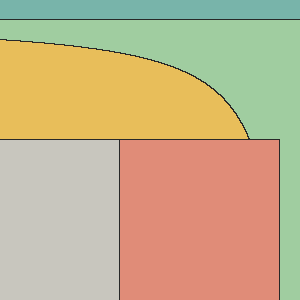
\includegraphics[width=7cm,height=7cm]{figures/rapport-carte-equilibres.png}};
\draw[black!50] (0,0) rectangle (1,1);
\foreach \t/\l in {0/0,0.2/20,0.4/40,0.6/60,0.8/80,1/100}{\draw (\t,0)--(\t,-0.015) node[below,font=\scriptsize]{\l\,\%};\draw (0,\t)--(-0.015,\t) node[left,font=\scriptsize]{\l\,\%};}
\draw[gov,line width=2.2pt] (0.5,0.5333)--(0.5,0.8);
\draw[gov,line width=2.2pt] (0,0.6)--(0.8,0.6);
\fill[gov] (0.5,0.6) circle (3pt); \draw[white,line width=1pt] (0.5,0.6) circle (3pt);
\node[font=\small,below] at (0.5,-0.08) {$q$ : le juge local refuse la censure};
\node[font=\small,rotate=90,above] at (-0.12,0.5) {$p$ : la Cour suprême donne raison aux journaux};
\node[anchor=west,font=\small,align=left] at (1.08,0.62) {%
\textcolor{cboth}{\rule{9pt}{9pt}} Deux procès : 1971 ($O_1$)\\[3pt]
\textcolor{cnyt}{\rule{9pt}{9pt}} Procès du Times seulement ($O_3$)\\[3pt]
\textcolor{cnosuit}{\rule{9pt}{9pt}} Publication sans procès ($O_4$)\\[3pt]
\textcolor{cnc}{\rule{9pt}{9pt}} Sans procès, menace non crédible\\[3pt]
\textcolor{cnone}{\rule{9pt}{9pt}} Rien ne sort ($O_7$)\\[8pt]
\textcolor{gov}{$\bullet$} nos valeurs : $q=50\,\%$, $p=60\,\%$\\
\textcolor{gov}{\rule[2pt]{14pt}{2pt}} intervalles du scénario de 1971};
\end{tikzpicture}
\caption{Pour chaque couple ($q$, $p$), l'issue de l'équilibre, les autres valeurs restant celles du groupe.}
\end{figure}
Lecture : si la Cour suprême est peu favorable ($p<53{,}3\,\%$), le Post n'ose pas prendre le relais. Selon le juge local, le Times publie alors seul ($O_3$) ou renonce ($O_7$). Si elle est très favorable ($p\ge80\,\%$), Nixon renonce au procès ($O_4$).

\subsection{L'intervalle du scénario de 1971}
Avec les formules de la fiche, $F=15$, $\tau_T=40\,\%$ et $\tau_W=53{,}3\,\%$ :
\begin{align*}
p \text{ pour } q=50\,\% :\quad & \max\!\Big(\tau_W\ ;\ \frac{\tau_T-q}{1-q}\Big)\le p<1-\frac{k_W+\frac{k_T}{1-q}}{F}
\ \Longrightarrow\ \boxed{\ 53{,}3\,\%\le p<1-\frac{1+2}{15}=80\,\%\ }\\[4pt]
q \text{ pour } p=60\,\% :\quad & \frac{\tau_T-p}{1-p}\le q<1-\frac{k_T}{(1-p)F-k_W}
\ \Longrightarrow\ \boxed{\ 0\le q<1-\frac{1}{6-1}=80\,\%\ }
\end{align*}

\begin{reponse}
\textbf{Les journaux publient} si leur chance de gagner dépasse leur seuil : le Post en relais si $p\ge53{,}3\,\%$ (seul : $q\ge53{,}3\,\%$) ; le Times si $q+(1-q)p\ge40\,\%$ quand il compte sur le relais du Post. Avec $q=50\,\%$ et $p=60\,\%$, les deux publient ; seul, le Post n'oserait pas.

\textbf{L'administration attaque} si le procès coûte moins que ce qu'il lui évite : contre le Post si $p<93{,}3\,\%$ ; contre le Times si $q<80\,\%$ (pour $p=60\,\%$). Le coût total espéré des procédures ($1{,}5$) est inférieur au gain espéré de la censure ($3$) : elle attaque. Si $k_T>2{,}5$ ou $k_W>4$, elle renonce et tout sort.

\textbf{Scénario de 1971} : $53{,}3\,\%\le p<80\,\%$ pour $q=50\,\%$ ; $q<80\,\%$ pour $p=60\,\%$.
\end{reponse}

% =====================================================================
\section{Consigne 4 : quand les documents ne sont-ils pas publiés ?}

Rien ne sort ($O_7$) si le Times renonce \emph{et} si le Post n'ose pas publier seul. Il faut donc que publier soit trop risqué pour le Times, alors que le Post seul ne publie déjà pas ($q=50\,\%<53{,}3\,\%$).

\subsection{Quatre cas chiffrés}
\begin{center}
\small
\begin{tabularx}{\textwidth}{@{}>{\raggedright\arraybackslash}p{3.3cm}cX@{}}
\toprule
Valeurs changées & Issue & Pourquoi les documents ne sortent pas \\
\midrule
\textbf{Tribunaux hostiles} : $q=20\,\%$, $p=30\,\%$ & $O_7$ & Le Post en relais perdrait ($p=30\,\%<53{,}3\,\%$ : gain $-2{,}8$). Le Times, alors seul face au juge local, n'a que $20\,\%<40\,\%$ de chances : publier lui rapporterait $0{,}2\times9+0{,}8\times(-6)=-3<0$. Le Post seul : $0{,}2\times7+0{,}8\times(-8)=-5<0$. Personne ne publie. \\
\addlinespace
\textbf{Sanction lourde pour le Times} : $S_T=40$ & $O_7$ & Son seuil monte à $\frac{1+40}{10+40}=82\,\%$, au-dessus de sa chance $\pi=80\,\%$ : publier lui rapporterait $0{,}8\times9+0{,}2\times(-41)=-1<0$. Le Post seul se tait ($-0{,}5$). Le seuil est $S_T>35$. \\
\addlinespace
\textbf{Procès coûteux pour le Times} : $c_T=9$ & $O_7$ & Seuil $\frac{9+5}{15}=93{,}3\,\%>80\,\%$ : gain $0{,}8\times1+0{,}2\times(-14)=-2<0$. Le seuil est $c_T>7$. \\
\addlinespace
\textbf{Le Post prend peur} : $c_W=5$ (ou $p=50\,\%$) & $O_3$ & Seuil du Post $\frac{5+5}{15}=66{,}7\,\%>60\,\%$ : il se tait. Le Times publie seul ($1{,}5>0$), Nixon le poursuit et la censure tient dans \textbf{$50\,\%$ des cas} : le secret est gardé une fois sur deux. \\
\bottomrule
\end{tabularx}
\end{center}

\begin{figure}[H]
\centering
\strip{Sanction du Times, $S_T$}{60}{0/35/cboth/1971,35/60/cnone/rien ne sort ($O_7$)}{5}

\medskip
\strip{Coût du procès du Times, $c_T$}{12}{0/7/cboth/1971,7/12/cnone/rien ne sort ($O_7$)}{1}

\medskip
\strip{Coût du procès du Post, $c_W$}{8}{0/4/cboth/1971,4/8/cnyt/procès du Times seul ($O_3$)}{3}

\medskip
\strip{Sanction du Post, $S_W$}{30}{0/7.5/cboth/1971,7.5/30/cnyt/procès du Times seul ($O_3$)}{5}
\caption{L'issue selon les coûts des journaux, les autres valeurs restant celles du groupe. Trait rouge : la valeur du groupe.}
\end{figure}

\subsection{L'importance des coûts des actions en justice}
Les coûts jouent dans les \textbf{deux sens} :
\begin{itemize}[leftmargin=*,itemsep=3pt]
\item \textbf{Coûts des journaux} ($c$, $S$) élevés : le seuil $\tau$ monte, les journaux se taisent et le secret est gardé ($O_7$), ou à moitié ($O_3$). La sanction $S$ pèse plus que les frais $c$, car elle ne tombe que si le journal perd mais efface tout son bénéfice.
\item \textbf{Coûts de Nixon} ($k_T$, $k_W$) élevés : les procès ne valent plus leur prix, Nixon laisse faire et \emph{tout sort} ($O_4$). Le coût du \emph{second} procès compte dès le premier : Nixon renonce à poursuivre le Times dès que $k_W>4$, alors que poursuivre le Post seul resterait rentable jusqu'à $6$.
\item \textbf{Ce que Nixon gagne à garder le secret} ($D+R$) : sans le bonus ($R=0$), $F=5$ et le premier procès ne rapporte que $0{,}5\times0{,}4\times5=1<1{,}5$. Nixon laisse faire, et tout sort ($O_4$). Le scénario de 1971 demande $R>2{,}5$.
\end{itemize}
\centerline{\strip{Bonus de Nixon si le secret est gardé, $R$}{20}{0/2.5/cnosuit/$O_4$,2.5/20/cboth/1971 : deux procès}{10}}

\begin{discuter}
\textbf{Menace non crédible.} Nixon pourrait \emph{annoncer} qu'il poursuivra tout le monde. Mais si un procès lui coûte plus qu'il ne lui rapporte (par exemple $k_W>6$), il ne l'exécuterait pas le moment venu : les journaux ne le croient pas. C'est pour cela que le coût des procès protège la presse.
\end{discuter}

\begin{reponse}
Les documents ne sont pas publiés ($O_7$) quand le Times renonce et que le Post n'ose pas publier seul : tribunaux hostiles ($q=20\,\%$, $p=30\,\%$), sanction du Times trop lourde ($S_T>35$) ou procès trop coûteux pour lui ($c_T>7$). Si seul le Post prend peur ($c_W>4$, $S_W>7{,}5$ ou $p<53{,}3\,\%$), le Times publie seul et le secret tient une fois sur deux ($O_3$). Des coûts élevés pour les journaux favorisent le secret. Des coûts élevés pour Nixon ($k_T>2{,}5$, $k_W>4$) rendent les procès non rentables, et tout sort.
\end{reponse}

% =====================================================================
\section{Consigne 5 : des gains cohérents et l'ENPS}

\subsection{Des gains cohérents avec les objectifs}
On classe les situations de la meilleure à la pire pour chaque joueur :
\begin{itemize}[leftmargin=*,itemsep=2pt]
\item \T{\textbf{Times}} : publier sans procès ($10$) $>$ gagner son procès ($9$) $>$ ne pas publier ($0$) $>$ perdre ($-6$).
\item \W{\textbf{Post}} : publier sans procès ($10$) $>$ gagner son procès ($7$) $>$ ne pas publier ($0$) $>$ perdre ($-8$).
\item \N{\textbf{Nixon}} : rien ne sort ($10$) $>$ censure obtenue après un ou deux procès ($9$, $8$) $>$ tout sort sans procès ($-5$) $>$ tout sort après un ou deux procès ($-6$, $-7$).
\end{itemize}
Chaque classement correspond à l'objectif du joueur : publier pour les journaux, garder le secret au moindre coût pour Nixon.

\subsection{Des gains cohérents entre les sous-jeux}
Un \emph{sous-jeu} commence à un nœud et contient toute la suite. Les gains sont cohérents parce que \textbf{chaque joueur n'a qu'une seule règle de calcul}, appliquée partout. Par exemple, « le Post gagne son procès » vaut toujours $7$, qu'il ait publié seul ou en relais ; « le Times ne publie pas » vaut toujours $0$ ($O_5$, $O_6$, $O_7$).

\begin{landscape}
\begin{center}{\large\bfseries Arbre 2 : les gains avec les valeurs du groupe, et l'équilibre}\\[2pt]{\small Gains dans l'ordre \textcolor{nyt}{\textbf{Times}}, \textcolor{wp}{\textbf{Post}}, \textcolor{gov}{\textbf{Nixon}}. $q$ = juge local, $p$ = Cour suprême. Poids des verdicts : $0{,}5$ ; $0{,}3$ ; $0{,}2$ (deux procès) et $0{,}5$ ; $0{,}5$ (un procès). Traits rouges épais : choix d'équilibre.}\end{center}\vspace{-4pt}
\noindent\resizebox{\linewidth}{!}{\begin{tikzpicture}[x=1cm,y=1cm,lab/.style={font=\scriptsize,fill=white,inner sep=1pt,sloped},eq/.style={line width=1.8pt,draw=gov},br/.style={line width=0.6pt,draw=black!55}]
\draw[eq] (0.4,-7.928125)--(2.6,-4.56875) node[lab,midway,above]{Publier};
\draw[br] (0.4,-7.928125)--(5.0,-11.2875) node[lab,midway,below]{Ne pas publier};
\draw[eq] (2.6,-4.56875)--(5.0,-2.6875) node[lab,midway,above]{Poursuivre};
\draw[br] (2.6,-4.56875)--(9.6,-6.449999999999999) node[lab,midway,below]{Laisser faire};
\draw[eq] (5.0,-2.6875)--(7.4,-1.075) node[lab,midway,above]{Publier};
\draw[br] (5.0,-2.6875)--(9.6,-4.3) node[lab,midway,below]{Ne pas publier};
\draw[eq] (7.4,-1.075)--(9.6,0.0) node[lab,midway,above]{Poursuivre};
\draw[br] (7.4,-1.075)--(9.6,-2.15) node[lab,midway,below]{Laisser faire};
\draw[br] (5.0,-11.2875)--(7.4,-9.675) node[lab,midway,above]{Publier};
\draw[eq] (5.0,-11.2875)--(9.6,-12.899999999999999) node[lab,midway,below]{Ne pas publier};
\draw[eq] (7.4,-9.675)--(9.6,-8.6) node[lab,midway,above]{Poursuivre};
\draw[br] (7.4,-9.675)--(9.6,-10.75) node[lab,midway,below]{Laisser faire};
\fill[nyt] (0.4,-7.928125) circle (4pt); \node[font=\small\bfseries,text=nyt,above left=3pt and -2pt] at (0.4,-7.928125) {Times};
\fill[gov] (2.6,-4.56875) circle (4pt); \node[font=\small\bfseries,text=gov,above left=3pt and -2pt] at (2.6,-4.56875) {Nixon};
\fill[wp] (5.0,-2.6875) circle (4pt); \node[font=\small\bfseries,text=wp,above left=3pt and -2pt] at (5.0,-2.6875) {Post};
\fill[gov] (7.4,-1.075) circle (4pt); \node[font=\small\bfseries,text=gov,above left=3pt and -2pt] at (7.4,-1.075) {Nixon};
\fill[wp] (5.0,-11.2875) circle (4pt); \node[font=\small\bfseries,text=wp,above left=3pt and -2pt] at (5.0,-11.2875) {Post};
\fill[gov] (7.4,-9.675) circle (4pt); \node[font=\small\bfseries,text=gov,above left=3pt and -2pt] at (7.4,-9.675) {Nixon};
\fill (9.6,0.0) circle (2pt);
\node[anchor=west,draw=black!35,fill=white,rounded corners=3pt,text width=15.2cm,align=left,font=\footnotesize,inner sep=4pt] at (9.85,0.0) {\textbf{$O_1$ · les deux journaux poursuivis}\\\textcolor{nyt}{\textbf{Times} : $0{,}5\times9+0{,}3\times9+0{,}2\times(-6)$ $=\mathbf{6}$}\\\textcolor{wp}{\textbf{Post} : $0{,}5\times0+0{,}3\times7+0{,}2\times(-8)$ $=\mathbf{0{,}5}$}\\\textcolor{gov}{\textbf{Nixon} : $0{,}5\times(-6)+0{,}3\times(-7)+0{,}2\times8$ $=\mathbf{-3{,}5}$}};
\fill (9.6,-2.15) circle (2pt);
\node[anchor=west,draw=black!35,fill=white,rounded corners=3pt,text width=15.2cm,align=left,font=\footnotesize,inner sep=4pt] at (9.85,-2.15) {\textbf{$O_2$ · Times poursuivi, Post libre}\\\textcolor{nyt}{\textbf{Times} : $10-1$ $=\mathbf{9}$}\\\textcolor{wp}{\textbf{Post} : $0{,}5\times0+0{,}5\times10$ $=\mathbf{5}$}\\\textcolor{gov}{\textbf{Nixon} : $-5-1$ $=\mathbf{-6}$}};
\fill (9.6,-4.3) circle (2pt);
\node[anchor=west,draw=black!35,fill=white,rounded corners=3pt,text width=15.2cm,align=left,font=\footnotesize,inner sep=4pt] at (9.85,-4.3) {\textbf{$O_3$ · Times poursuivi, Post muet}\\\textcolor{nyt}{\textbf{Times} : $0{,}5\times9+0{,}5\times(-6)$ $=\mathbf{1{,}5}$}\\\textcolor{wp}{\textbf{Post} : $\mathbf{0}$}\\\textcolor{gov}{\textbf{Nixon} : $0{,}5\times(-6)+0{,}5\times9$ $=\mathbf{1{,}5}$}};
\fill (9.6,-6.449999999999999) circle (2pt);
\node[anchor=west,draw=black!35,fill=white,rounded corners=3pt,text width=15.2cm,align=left,font=\footnotesize,inner sep=4pt] at (9.85,-6.449999999999999) {\textbf{$O_4$ · Times publie, pas de procès}\\\textcolor{nyt}{\textbf{Times} : $\mathbf{10}$}\\\textcolor{wp}{\textbf{Post} : $\mathbf{0}$}\\\textcolor{gov}{\textbf{Nixon} : $\mathbf{-5}$}};
\fill (9.6,-8.6) circle (2pt);
\node[anchor=west,draw=black!35,fill=white,rounded corners=3pt,text width=15.2cm,align=left,font=\footnotesize,inner sep=4pt] at (9.85,-8.6) {\textbf{$O_5$ · Post seul, poursuivi}\\\textcolor{nyt}{\textbf{Times} : $\mathbf{0}$}\\\textcolor{wp}{\textbf{Post} : $0{,}5\times7+0{,}5\times(-8)$ $=\mathbf{-0{,}5}$}\\\textcolor{gov}{\textbf{Nixon} : $0{,}5\times(-6)+0{,}5\times9$ $=\mathbf{1{,}5}$}};
\fill (9.6,-10.75) circle (2pt);
\node[anchor=west,draw=black!35,fill=white,rounded corners=3pt,text width=15.2cm,align=left,font=\footnotesize,inner sep=4pt] at (9.85,-10.75) {\textbf{$O_6$ · Post seul, pas de procès}\\\textcolor{nyt}{\textbf{Times} : $\mathbf{0}$}\\\textcolor{wp}{\textbf{Post} : $\mathbf{10}$}\\\textcolor{gov}{\textbf{Nixon} : $\mathbf{-5}$}};
\fill (9.6,-12.899999999999999) circle (2pt);
\node[anchor=west,draw=black!35,fill=white,rounded corners=3pt,text width=15.2cm,align=left,font=\footnotesize,inner sep=4pt] at (9.85,-12.899999999999999) {\textbf{$O_7$ · personne ne publie}\\\textcolor{nyt}{\textbf{Times} : $\mathbf{0}$}\\\textcolor{wp}{\textbf{Post} : $\mathbf{0}$}\\\textcolor{gov}{\textbf{Nixon} : $\mathbf{10}$}};
\end{tikzpicture}}
\end{landscape}


\subsection{La résolution par induction à rebours}
On part des derniers nœuds et on remonte. À chaque nœud, le joueur garde l'action qui lui rapporte le plus. À égalité, un journal publie et Nixon ne poursuit pas.
\begin{center}
\small
\begin{tabular}{@{}clll@{}}
\toprule
Nœud & Qui décide & Comparaison & Choix \\
\midrule
$x_3$ & \N{Nixon} face au Post & poursuivre ($O_1$) : $-3{,}5$ \ contre \ laisser faire ($O_2$) : $-6$ & poursuivre \\
$x_2$ & \W{Post} en relais & publier ($O_1$) : $0{,}5$ \ contre \ se taire ($O_3$) : $0$ & publier \\
$x_1$ & \N{Nixon} face au Times & poursuivre ($O_1$) : $-3{,}5$ \ contre \ laisser faire ($O_4$) : $-5$ & poursuivre \\
$x_5$ & \N{Nixon} face au Post seul & poursuivre ($O_5$) : $1{,}5$ \ contre \ laisser faire ($O_6$) : $-5$ & poursuivre \\
$x_4$ & \W{Post} seul & publier ($O_5$) : $-0{,}5$ \ contre \ se taire ($O_7$) : $0$ & se taire \\
$x_0$ & \T{Times} & publier ($O_1$) : $6$ \ contre \ se taire ($O_7$) : $0$ & publier \\
\bottomrule
\end{tabular}
\end{center}

\subsection{L'ENPS et son résultat}
\begin{center}
\small
\begin{tabular}{@{}ll@{}}
\toprule
Joueur & Stratégie d'équilibre (un choix à chacun de ses nœuds) \\
\midrule
\T{Times} & publier \\
\W{Post} & publier en relais ($x_2$) ; se taire s'il est seul ($x_4$) \\
\N{Nixon} & poursuivre le Times ($x_1$) ; poursuivre le Post en relais ($x_3$) ; poursuivre le Post seul ($x_5$) \\
\bottomrule
\end{tabular}
\end{center}

\begin{figure}[H]
\centering
\begin{tikzpicture}
\fill[wp!55] (0,0) rectangle (5,0.6); \node[font=\small\bfseries,white] at (2.5,0.3){A : juge local, $50\,\%$};
\fill[wp!80] (5,0) rectangle (8,0.6); \node[font=\small\bfseries,white] at (6.5,0.3){B : Cour, $30\,\%$};
\fill[gov!75] (8,0) rectangle (10,0.6); \node[font=\small\bfseries,white] at (9,0.3){C : $20\,\%$};
\draw[black!50] (0,0) rectangle (10,0.6);
\node[font=\scriptsize,below] at (4,-0.02){tout sort : $80\,\%$};
\draw[decorate,decoration={brace,mirror,amplitude=4pt}] (0,-0.05)--(8,-0.05);
\node[font=\scriptsize,below] at (9,-0.02){censure : $20\,\%$};
\end{tikzpicture}
\caption{Une fois à $O_1$, les juges tranchent : les documents finissent par sortir dans $80\,\%$ des cas. En 1971, c'est le verdict B (la Cour suprême, 6 voix contre 3).}
\end{figure}

\subsection{Pourquoi « parfait en sous-jeux » ?}
Sur les 64 profils de stratégies, \textbf{4 sont des équilibres de Nash}. Tous mènent à $O_1$ ; ils ne diffèrent que hors du chemin, aux nœuds $x_4$ et $x_5$ :
\begin{center}
\small
\begin{tabular}{@{}lll@{}}
\toprule
Post seul ($x_4$) & Nixon face au Post seul ($x_5$) & Parfait en sous-jeux ? \\
\midrule
se taire & poursuivre & \textbf{oui : l'ENPS} \\
publier & poursuivre & non : seul, publier lui rapporterait $-0{,}5<0$ \\
se taire & laisser faire & non : Nixon gagnerait $1{,}5>-5$ en poursuivant \\
publier & laisser faire & non : Nixon poursuivrait le moment venu \\
\bottomrule
\end{tabular}
\end{center}
Ces trois autres profils sont des équilibres de Nash parce que ces nœuds ne sont jamais atteints. L'ENPS exige en plus que chaque joueur fasse le bon choix \emph{dans chaque sous-jeu}, même hors du chemin : il élimine les menaces et promesses non crédibles.

\begin{reponse}
\textbf{Gains} : une seule règle par joueur ($u_j=B\sigma-c-S$ pour un journal, $0$ s'il ne publie pas ; $u_N=R(1-\sigma)-D\sigma-k_T-k_W$ pour Nixon), cohérente avec ses objectifs et identique dans tous les sous-jeux.

\textbf{ENPS} (unique) : le Times publie ; le Post publie en relais et se tait seul ; Nixon poursuit à ses trois nœuds. \textbf{Résultat} : $O_1$, procès contre les deux journaux, gains espérés $(6\ ;\ 0{,}5\ ;\ -3{,}5)$. Les documents sortent avec $80\,\%$ de chances. C'est l'histoire de 1971.
\end{reponse}

% =====================================================================
\section{Robustesse et limites}
\begin{itemize}[leftmargin=*,itemsep=2pt]
\item \textbf{Avec $\theta=0{,}3$} (les trois articles parus avant la censure) : encore 1971, avec $(6{,}6\ ;\ 1{,}1\ ;\ -4{,}4)$ ; l'intervalle devient $41{,}7\,\%\le p<71{,}4\,\%$ (pour $q=50\,\%$).
\item \textbf{Sans bonus mais avec un grand dommage} ($R=0$, $D=200$) : encore 1971. Le bonus $R$ joue le même rôle qu'un dommage plus grand : $R(1-\sigma)-D\sigma=R-(D+R)\sigma$.
\item Les valeurs sont des hypothèses : ce sont les \emph{seuils} qui répondent à l'énoncé.
\item La Cour suprême n'est saisie que si les deux journaux sont poursuivis ; tous les joueurs connaissent les gains et les probabilités (information complète) ; une seule affaire, pas un jeu répété.
\end{itemize}

\end{document}
